\section*{1. Timeline At A Glance}

The project changed direction a few times, but the main arc was fairly consistent: baseline recovery first, then stronger tree ensembles, then a target-stat branch, then neural or meta layers on top of those tabular sources, and finally a professor-inspired parallel lane to test whether broader feature generation could push the upstream score further.

\softpanel{ink}{%
\textbf{If you only want the short version}
\begin{itemize}
    \item The first reliable jump came from turning the baseline into a stronger tree ensemble, not from chasing exotic models too early.
    \item The most important classical step was the target-stats branch.
    \item The best local score came later from a neural or meta blend on top of strong tabular branches, not from abandoning those branches.
    \item The professor lane improved the refreshed target-stats source a little, but the strongest final local blends still came from the already strong hybrid stack.
\end{itemize}}

\begin{figure}[H]
    \centering
    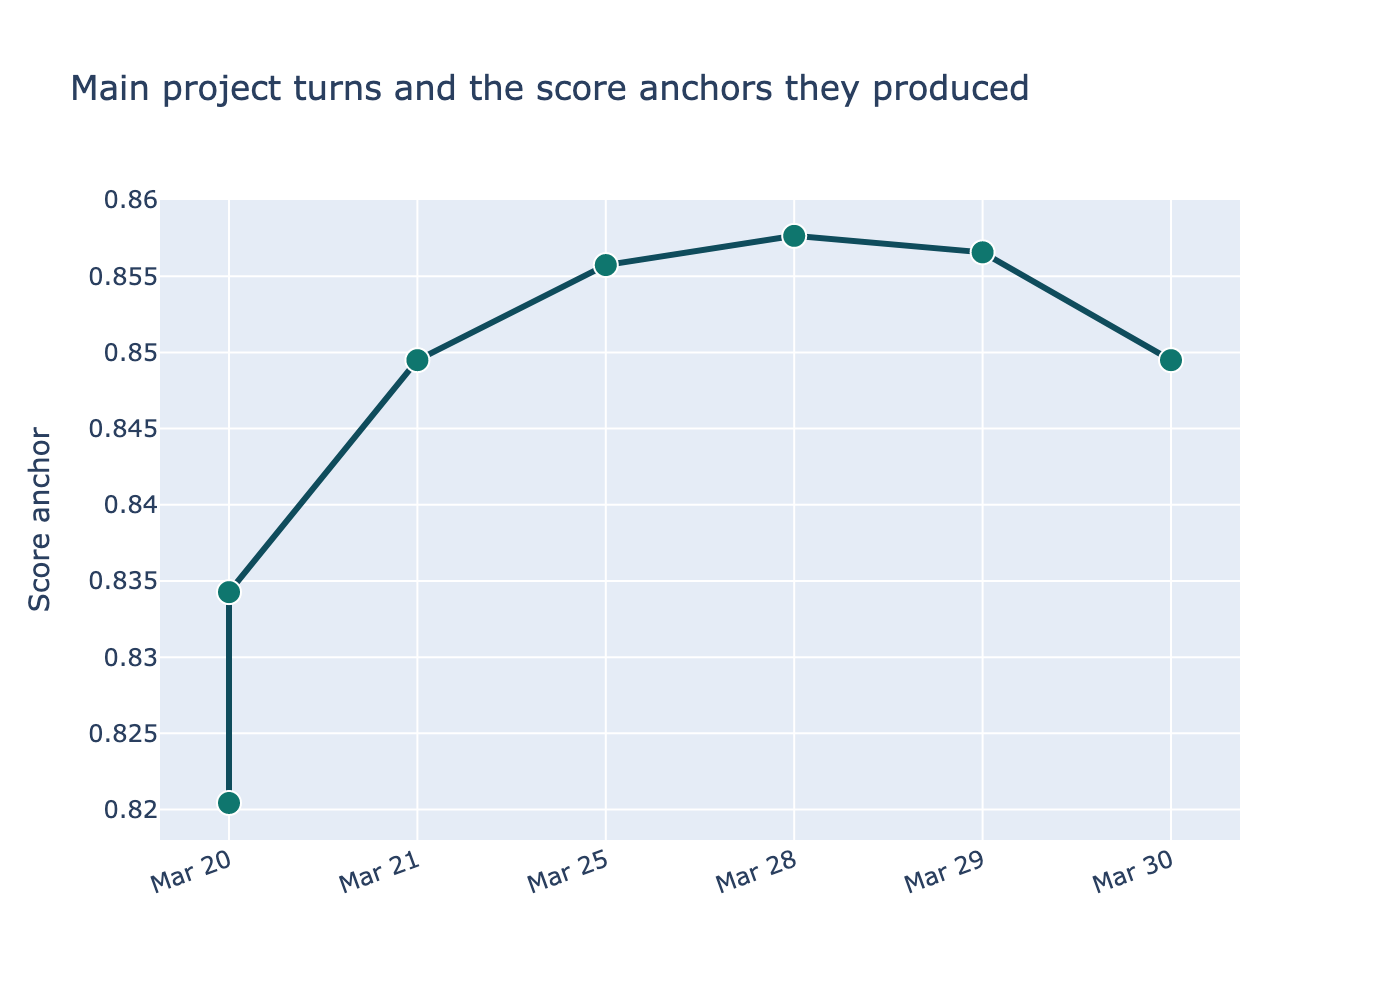
\includegraphics[width=\linewidth]{figures/methods_milestones.png}
    \caption{The main turns in the project, shown with the score anchor each phase produced.}
\end{figure}

\rowcolors{2}{coolbg}{white}
\begin{table}[H]
    \centering
    \small
    \begin{tabularx}{\linewidth}{>{\bfseries}p{0.13\linewidth} >{\raggedright\arraybackslash}p{0.22\linewidth} >{\centering\arraybackslash}p{0.12\linewidth} X}
        \rowcolor{ink!12}
        Date & Phase & Score & What changed \\
        Mar 20 & Baseline reconstruction & 0.82043 public & Recovered the assignment setup, rebuilt the baseline, and used the first Kaggle checks to calibrate the local split. \\
        Mar 20 & Poly-parallel tree blend & 0.834266 & The baseline turned into a broader tree stack, with an extra MPS-supported lane. \\
        Mar 21 & Overnight ensemble & 0.849489 & Tuned XGB, LGB, CatBoost, ExtraTrees, and MPS were combined into the first really systematic ensemble family. \\
        Mar 25 & Target-stats branch & 0.855731 & OOF target statistics and stronger pruning pushed the main classical branch into the mid 0.855 range. \\
        Mar 28 & Neural and meta topping & 0.857645 & The best local score came from a weighted neural/meta blend placed on top of strong tabular branches rather than a fully neural replacement. \\
        Mar 29 & Professor lane & 0.856566 & Broader feature generation and a refreshed target-stats branch improved the upstream source a bit, but did not replace the strongest final blends. \\
        Mar 30 & Public packaging & 0.849489 & The public repo was rebuilt around the cleaner overnight lane because it stayed reproducible and easy to explain. \\
    \end{tabularx}
    \caption{The seven project turns that matter most to the final story.}
\end{table}

Two practical notes shaped the work from early on. First, Kaggle submissions were treated as scarce calibration points rather than as blind search. Second, the repo became dense quickly, so each later stage was judged not only by score, but also by whether it stayed understandable enough to package into a clean final deliverable.
